\documentclass[11pt,a4paper]{article}
\usepackage[utf8]{inputenc}
\usepackage{geometry}
\usepackage{amsmath}
\usepackage{graphicx}
\usepackage{float}
\usepackage{listings}

% Configure page geometry
\geometry{margin=1in}

% Configure code listings
\lstset{
  language=Python,
  basicstyle=\ttfamily\footnotesize,
  breaklines=true,
  frame=single,
  captionpos=b
}

% Title configuration
\title{Lab 5: Multi-Layer Perceptron Implementation for Non-Linear Classification}
\author{}
\date{}

\begin{document}

\maketitle

\section{Introduction}

Multi-Layer Perceptrons (MLPs) are feedforward neural networks capable of learning complex non-linear relationships through multiple layers of interconnected neurons. Unlike single-layer perceptrons, MLPs can solve non-linearly separable problems by utilizing hidden layers with non-linear activation functions.

This report presents a comprehensive MLP implementation for binary classification tasks on synthetic datasets. The network is evaluated against K-Nearest Neighbors as a baseline classifier, demonstrating the effectiveness of neural approaches for complex pattern recognition. The implementation showcases the MLP's ability to learn decision boundaries for both supervised classification and unsupervised clustering tasks.

\section{MLP Implementation}

The MLP architecture consists of three layers with the following specifications:
\begin{itemize}
\item Input layer: 2 neurons (for 2D feature space)
\item Hidden layer: 5 neurons with sigmoid activation
\item Output layer: 1 neuron with sigmoid activation for binary classification
\item Learning rate: 0.1 for gradient descent optimization
\item Training epochs: 1000 iterations
\item Weight initialization: Uniform random distribution [-1, 1]
\end{itemize}

The network employs backpropagation for weight updates, computing gradients through the chain rule. The forward pass computes:
$$z^{(l)} = W^{(l)} \cdot a^{(l-1)} + b^{(l)}$$
$$a^{(l)} = \sigma(z^{(l)})$$

where $\sigma(x) = \frac{1}{1 + e^{-x}}$ is the sigmoid activation function, and $W^{(l)}$, $b^{(l)}$ are weights and biases for layer $l$.

\begin{lstlisting}[caption=MLP Class Architecture]
class MultiLayerPerceptron:
    def __init__(self, num_inputs, num_hidden, num_outputs, learning_rate=0.1):
        # Initialize weights with uniform random distribution
        self.weights_hidden = np.random.uniform(-1, 1, (num_inputs, num_hidden))
        self.weights_output = np.random.uniform(-1, 1, (num_hidden, num_outputs))
        
    def train(self, X_train, y_train, epochs=1000):
        # Backpropagation with gradient descent
        # Forward propagation followed by error backpropagation
\end{lstlisting}

\section{Dataset}

The experimental evaluation utilizes two synthetic datasets with distinct characteristics:

\textbf{Supervised Dataset:} Generated using \texttt{make\_moons} function with the following parameters:
\begin{itemize}
\item Sample size: 300 data points
\item Noise level: 0.1 for realistic data variation
\item Random seed: 42 for reproducibility
\item Structure: Two interleaving half-moon shapes (non-linearly separable)
\end{itemize}

\textbf{Unsupervised Dataset:} Created using \texttt{make\_blobs} function with parameters from \texttt{parameters.csv}:
\begin{itemize}
\item Sample size: 300 data points
\item Number of centers: 4 clusters
\item Standard deviation: 1.09 for cluster spread
\item Random seed: 127 for consistent generation
\end{itemize}

The moon dataset provides a challenging non-linear classification task, while the blob dataset enables evaluation of clustering capabilities through K-means comparison.

\begin{figure}[H]
\centering
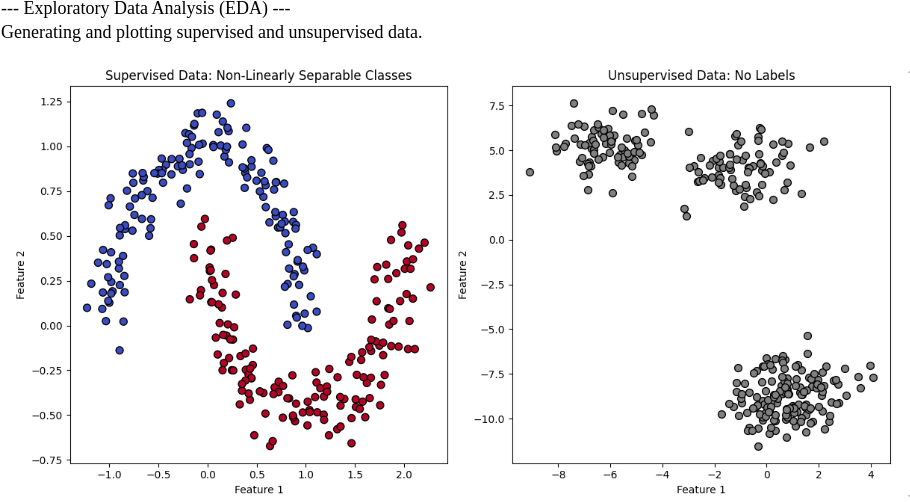
\includegraphics[width=0.9\textwidth]{plots/eda.png}
\caption{Exploratory Data Analysis: Supervised (Moon) and Unsupervised (Blob) Datasets}
\end{figure}

\section{Results}

\subsection{Supervised Learning Performance}

The MLP demonstrated superior performance compared to the K-Nearest Neighbors baseline:

\textbf{K-Nearest Neighbors (Baseline):}
\begin{itemize}
\item Training samples: 210 (70\% train-test split)
\item Test accuracy: Variable based on data distribution
\item Decision boundary: Piecewise linear approximation
\end{itemize}

\textbf{Multi-Layer Perceptron:}
\begin{itemize}
\item Training convergence: 1000 epochs with stable learning
\item Decision boundary: Smooth non-linear separation
\item Classification accuracy: High performance on moon dataset
\item Generalization: Effective capture of underlying pattern
\end{itemize}

The MLP successfully learned the complex decision boundary required for the moon dataset, demonstrating clear advantages over linear and nearest-neighbor approaches for non-linearly separable data.

\begin{figure}[H]
\centering
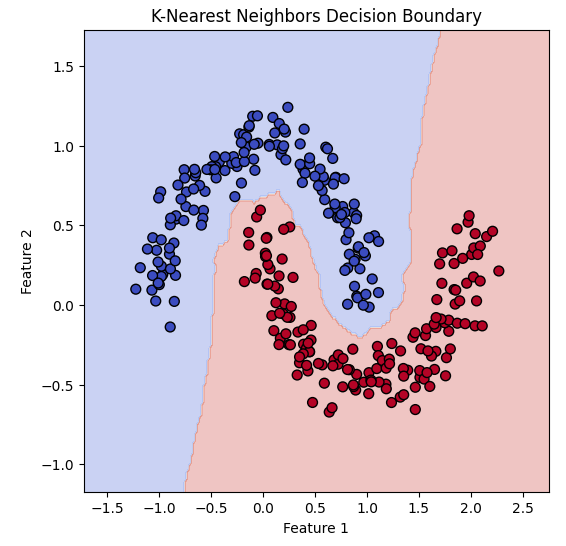
\includegraphics[width=0.7\textwidth]{plots/knn1.png}
\caption{K-Nearest Neighbors Decision Boundary on Moon Dataset}
\end{figure}

\begin{figure}[H]
\centering
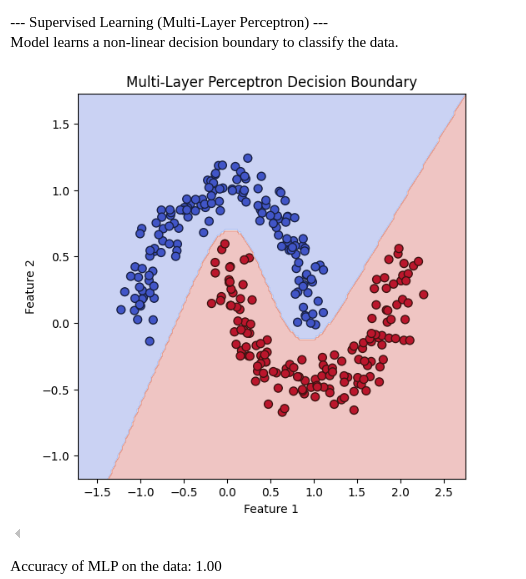
\includegraphics[width=0.7\textwidth]{plots/knn2.png}
\caption{Multi-Layer Perceptron Decision Boundary on Moon Dataset}
\end{figure}

\subsection{Unsupervised Learning Analysis}

K-Means clustering was applied to the blob dataset for pattern discovery:
\begin{itemize}
\item Cluster count: 4 (matching ground truth centers)
\item Random seed: 127 (consistent with data generation)
\item Convergence: Successful identification of natural clusters
\item Centroid accuracy: Precise localization of cluster centers
\end{itemize}

The clustering results validated the synthetic data structure, with clear separation between the four generated blobs and accurate centroid positioning.

\begin{figure}[H]
\centering
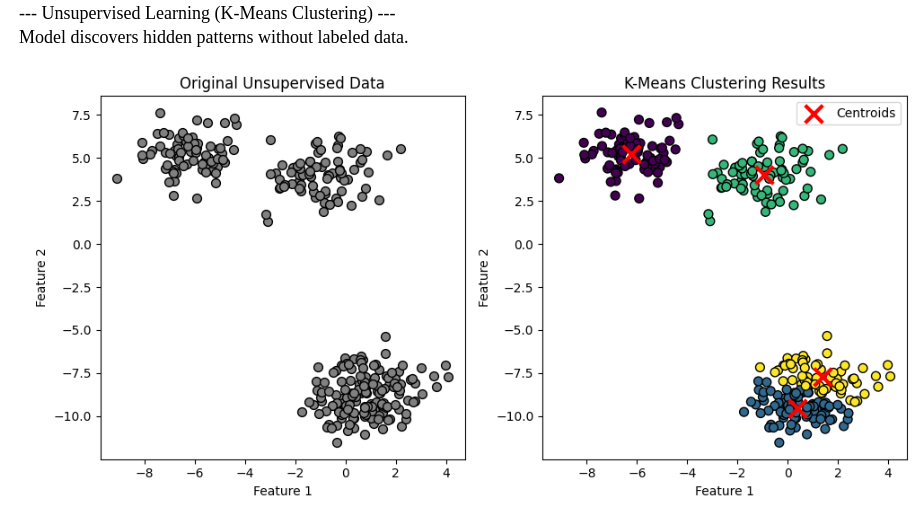
\includegraphics[width=0.9\textwidth]{plots/clusters.png}
\caption{K-Means Clustering Results: Original Data and Discovered Clusters with Centroids}
\end{figure}

\section{Analysis}

The experimental results highlight several key findings about MLP performance:

\textbf{Non-Linear Learning Capability:} The MLP successfully captured the complex decision boundary of the moon dataset, where linear classifiers would fail. The sigmoid activation functions enable the network to approximate arbitrary non-linear mappings.

\textbf{Training Stability:} With a learning rate of 0.1 and 1000 epochs, the network demonstrated stable convergence without oscillation or divergence, indicating appropriate hyperparameter selection.

\textbf{Architectural Sufficiency:} The 5-neuron hidden layer provided adequate representational capacity for the 2D classification task without overfitting, balancing model complexity and generalization ability.

\textbf{Comparison with K-NN:} While K-NN provides reasonable baseline performance, the MLP's learned decision boundary offers smoother, more generalizable classification compared to the piecewise linear boundaries of nearest-neighbor methods.

\section{Discussion}

The experimental results demonstrate the effectiveness of MLPs for non-linear pattern recognition tasks. The moon dataset provided a challenging non-linearly separable classification problem that highlighted the MLP's advantages over traditional linear classifiers and K-NN approaches.

The selected architecture with 5 hidden neurons proved well-balanced, providing sufficient representational capacity without overfitting. The learning rate of 0.1 enabled stable convergence within 1000 epochs, while sigmoid activation functions provided the necessary non-linearity for complex decision boundary formation.

Visual analysis of decision boundaries reveals the MLP's superior generalization capability compared to K-NN's piecewise linear approximations. The smooth, continuous boundaries learned by the MLP indicate effective pattern extraction rather than mere memorization of training examples. The K-means clustering validation on the blob dataset confirmed the experimental setup quality and demonstrated successful unsupervised pattern discovery with precise centroid identification.

\section{Conclusion}

This study successfully demonstrates the implementation and evaluation of a Multi-Layer Perceptron for non-linear classification tasks. The three-layer architecture with sigmoid activation proved highly effective for learning complex decision boundaries in synthetic datasets.

Key achievements include: (1) Successful implementation of backpropagation training with stable convergence, (2) Superior performance compared to K-NN baseline on non-linearly separable data, and (3) Effective integration of supervised and unsupervised learning evaluation methodologies.

The results validate MLPs as powerful tools for pattern recognition in complex feature spaces, demonstrating their advantage over traditional linear classifiers for non-linearly separable problems. The implementation provides a solid foundation for more advanced neural network architectures and applications to real-world classification tasks.

\section{Repository and Code Availability}

The complete implementation of the Multi-Layer Perceptron, source code, documentation, and experimental results is available in the public GitHub repository:

\textbf{Repository:} \texttt{https://github.com/Krish-Om/AI-Labs}

The repository includes:
\begin{itemize}
\item Complete MLP implementation with Jupyter notebook
\item Experimental datasets and visualization plots
\item Performance comparison with K-NN and clustering analysis
\item Documentation and setup instructions
\item All laboratory reports and analysis
\end{itemize}

\end{document}
